%
% randdef.tex
%
\begin{figure}
\centering
%\vspace*{2cm}
%XXX Glatter Rand eines Gebietes
%\vspace*{2cm}
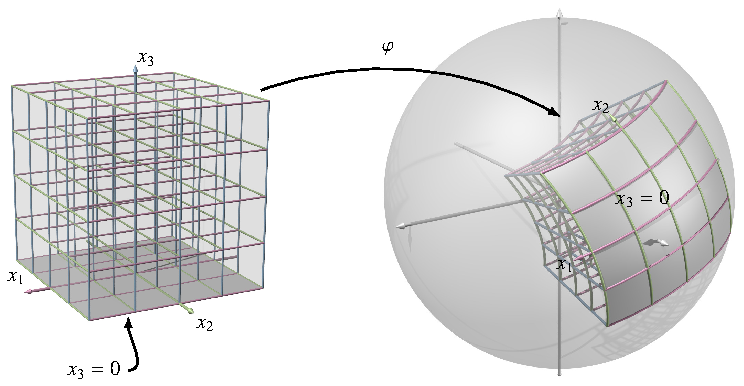
\includegraphics{chapters/040-felder/images/randdef.pdf}
\caption{Der Rand eines Gebietes heisst glatt, wenn jeder Punkt eine
Umgebung hat, die bijektiv und differenzierbar auf eine offene Umgebung
des Nullpunktes abgebildet werden kann, so dass die Hyperebene $x_n=0$
auf den Rand abgebildet wird.
\label{buch:felder:fundamentallemma:fig:randdef}}
\end{figure}
